\documentclass[12pt]{article}
\usepackage[margin=1in]{geometry}
\usepackage{graphicx}
\usepackage{verbatim}
\setlength{\parskip}{0.5em}

\title{Code, Quotation, and Imagery in Body Text}
\author{legible-pdf synthesized corpus}
\date{}

\begin{document}
\maketitle

\section{Source Code}

The following Python function implements binary search over a sorted sequence,
returning the index of the target value or $-1$ when no match is found.

\begin{verbatim}
def binary_search(arr, target):
    lo, hi = 0, len(arr) - 1
    while lo <= hi:
        mid = (lo + hi) // 2
        if arr[mid] == target:
            return mid
        elif arr[mid] < target:
            lo = mid + 1
        else:
            hi = mid - 1
    return -1
\end{verbatim}

The implementation uses zero-based indexing and the floor-division operator,
which are conventional in Python source.

\section{Quotation}

A frequently quoted observation about software construction comes from Donald
Knuth's writing on optimization.

\begin{quote}
Premature optimization is the root of all evil. We should forget about small
efficiencies, say about ninety-seven percent of the time.
\end{quote}

The full passage from Knuth continues with a qualifier that is often omitted
from popular paraphrases.

\section{Imagery}

A sample bar chart accompanies the text in Figure~\ref{fig:chart}, illustrating
how visual elements appear within a document body.

\begin{figure}[h]
\centering
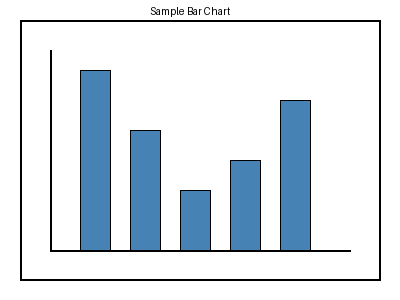
\includegraphics[width=0.5\textwidth]{chart.png}
\caption{A sample bar chart with five vertical bars.}
\label{fig:chart}
\end{figure}

As shown in Figure~\ref{fig:chart}, bars of varying heights occupy a plotted
region bounded by axis lines.

\section{Glossary}

The document mentions: a Python function named binary\_search, the operators
floor-division and equality, the integer return value $-1$, the author Donald
Knuth, the phrase premature optimization, and a bar chart figure with five
bars.

\end{document}
